\subsection{Psf\-Match  Class Reference}
\label{class_psfmatch}\index{PsfMatch@{Psf\-Match}}
A class that wraps calls to {\bf Kernel\-Fit} {\rm (p.\,\pageref{class_kernelfit})}. Used both to carry out subtractions ({\bf Image\-Subtraction} {\rm (p.\,\pageref{class_imagesubtraction})}) and just kernel fitting (for the light curve). 


{\tt \#include $<$psfmatch.h$>$}

Inheritance diagram for Psf\-Match::\begin{figure}[H]
\begin{center}
\leavevmode
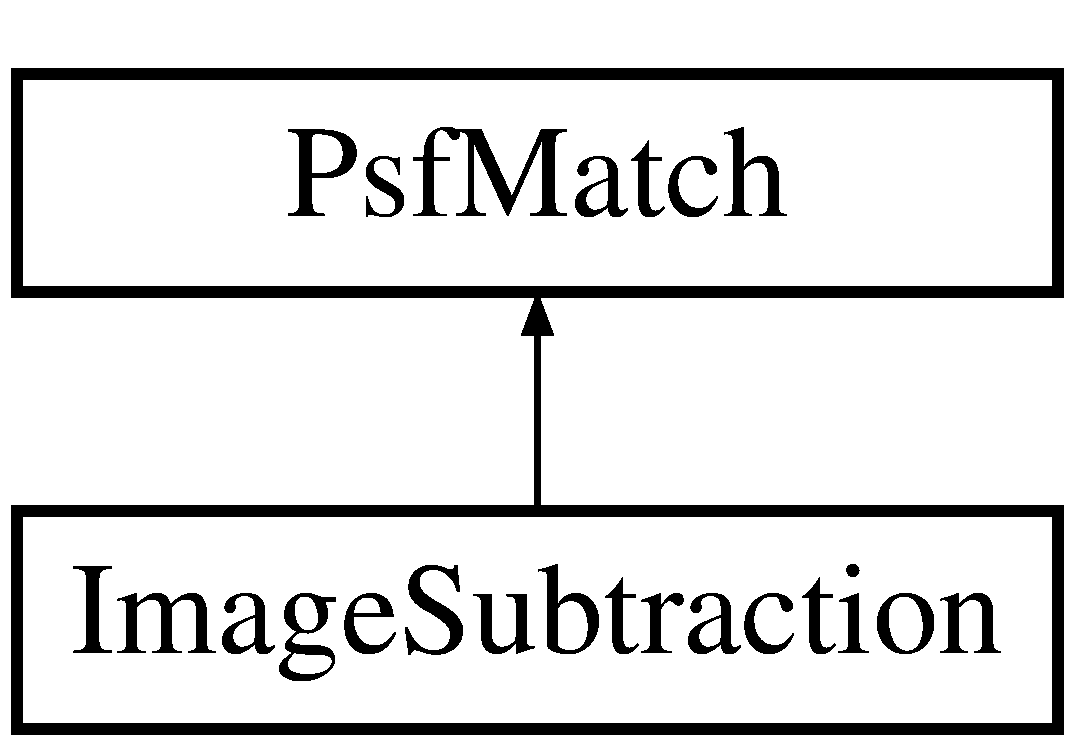
\includegraphics[height=2cm]{class_psfmatch}
\end{center}
\end{figure}
\subsubsection*{Public Methods}
\begin{CompactItemize}
\item 
\index{NotFilteredStarListName@{NotFilteredStarListName}!PsfMatch@{Psf\-Match}}\index{PsfMatch@{PsfMatch}!NotFilteredStarListName@{Not\-Filtered\-Star\-List\-Name}}
string {\bf Not\-Filtered\-Star\-List\-Name} ()\label{class_psfmatch_a0}

\item 
\index{PsfMatch@{PsfMatch}!PsfMatch@{Psf\-Match}}\index{PsfMatch@{PsfMatch}!PsfMatch@{Psf\-Match}}
{\bf Psf\-Match} (const {\bf Reduced\-Image} \&Ref, const {\bf Reduced\-Image} \&New, const Psf\-Match $\ast$APrevious\-Match=NULL)\label{class_psfmatch_a1}

\item 
\index{~PsfMatch@{$\sim$PsfMatch}!PsfMatch@{Psf\-Match}}\index{PsfMatch@{PsfMatch}!~PsfMatch@{$\sim$Psf\-Match}}
{\bf $\sim$Psf\-Match} ()\label{class_psfmatch_a2}

\item 
\index{PsfMatch@{PsfMatch}!PsfMatch@{Psf\-Match}}\index{PsfMatch@{PsfMatch}!PsfMatch@{Psf\-Match}}
{\bf Psf\-Match} (const Psf\-Match \&Original)\label{class_psfmatch_a3}

\item 
\index{PsfMatch@{PsfMatch}!PsfMatch@{Psf\-Match}}\index{PsfMatch@{PsfMatch}!PsfMatch@{Psf\-Match}}
{\bf Psf\-Match} ()\label{class_psfmatch_a4}

\item 
\index{FitKernel@{FitKernel}!PsfMatch@{Psf\-Match}}\index{PsfMatch@{PsfMatch}!FitKernel@{Fit\-Kernel}}
bool {\bf Fit\-Kernel} (const bool Keep\-Images=false)\label{class_psfmatch_a5}

\begin{CompactList}\small\item\em Carry out kernel fit. argument to enable to keep the images.\item\end{CompactList}\item 
\index{FilterStarList@{FilterStarList}!PsfMatch@{Psf\-Match}}\index{PsfMatch@{PsfMatch}!FilterStarList@{Filter\-Star\-List}}
int {\bf Filter\-Star\-List} (const double Max\-Dist=1)\label{class_psfmatch_a6}

\item 
\index{PhotomRatio@{PhotomRatio}!PsfMatch@{Psf\-Match}}\index{PsfMatch@{PsfMatch}!PhotomRatio@{Photom\-Ratio}}
double {\bf Photom\-Ratio} () const\label{class_psfmatch_a7}

\item 
\index{Chi2@{Chi2}!PsfMatch@{Psf\-Match}}\index{PsfMatch@{PsfMatch}!Chi2@{Chi2}}
double {\bf Chi2} () const\label{class_psfmatch_a8}

\item 
\index{SigmaBack@{SigmaBack}!PsfMatch@{Psf\-Match}}\index{PsfMatch@{PsfMatch}!SigmaBack@{Sigma\-Back}}
double {\bf Sigma\-Back} () const\label{class_psfmatch_a9}

\item 
\index{Intersection@{Intersection}!PsfMatch@{Psf\-Match}}\index{PsfMatch@{PsfMatch}!Intersection@{Intersection}}
{\bf Frame} {\bf Intersection} () const\label{class_psfmatch_a10}

\item 
\index{KernelToWorst@{KernelToWorst}!PsfMatch@{Psf\-Match}}\index{PsfMatch@{PsfMatch}!KernelToWorst@{Kernel\-To\-Worst}}
void {\bf Kernel\-To\-Worst} ({\bf Kernel} \&Result, const double \&x, const double \&y) const\label{class_psfmatch_a11}

\item 
\index{BackKernel@{BackKernel}!PsfMatch@{Psf\-Match}}\index{PsfMatch@{PsfMatch}!BackKernel@{Back\-Kernel}}
void {\bf Back\-Kernel} ({\bf Kernel} \&Diffback, const double \&xc, const double \&yc)\label{class_psfmatch_a12}

\item 
\index{VarianceConvolve@{VarianceConvolve}!PsfMatch@{Psf\-Match}}\index{PsfMatch@{PsfMatch}!VarianceConvolve@{Variance\-Convolve}}
bool {\bf Variance\-Convolve} ({\bf Image} \&Variance)\label{class_psfmatch_a13}

\begin{CompactList}\small\item\em builds the subtraction image new-ref (in photometric units of the ref). Puts it as the fits image of RImage. Sets seeing \& co. Does not keep by default the result of the convolution.\item\end{CompactList}\item 
\index{ConvolveBest@{ConvolveBest}!PsfMatch@{Psf\-Match}}\index{PsfMatch@{PsfMatch}!ConvolveBest@{Convolve\-Best}}
void {\bf Convolve\-Best} ({\bf Reduced\-Image} \&Conv\-Image)\label{class_psfmatch_a14}

\item 
\index{Subtraction@{Subtraction}!PsfMatch@{Psf\-Match}}\index{PsfMatch@{PsfMatch}!Subtraction@{Subtraction}}
bool {\bf Subtraction} ({\bf Reduced\-Image} \&RImage, bool Keep\-Convolved\-Best=false)\label{class_psfmatch_a15}

\item 
\index{RefIsBest@{RefIsBest}!PsfMatch@{Psf\-Match}}\index{PsfMatch@{PsfMatch}!RefIsBest@{Ref\-Is\-Best}}
bool {\bf Ref\-Is\-Best} () const\label{class_psfmatch_a16}

\item 
\index{Ref@{Ref}!PsfMatch@{Psf\-Match}}\index{PsfMatch@{PsfMatch}!Ref@{Ref}}
{\bf Reduced\-Image}$\ast$ {\bf Ref} ()\label{class_psfmatch_a17}

\item 
\index{New@{New}!PsfMatch@{Psf\-Match}}\index{PsfMatch@{PsfMatch}!New@{New}}
{\bf Reduced\-Image}$\ast$ {\bf New} ()\label{class_psfmatch_a18}

\item 
\index{Best@{Best}!PsfMatch@{Psf\-Match}}\index{PsfMatch@{PsfMatch}!Best@{Best}}
{\bf Reduced\-Image}$\ast$ {\bf Best} ()\label{class_psfmatch_a19}

\item 
\index{Worst@{Worst}!PsfMatch@{Psf\-Match}}\index{PsfMatch@{PsfMatch}!Worst@{Worst}}
{\bf Reduced\-Image}$\ast$ {\bf Worst} ()\label{class_psfmatch_a20}

\end{CompactItemize}
\subsubsection*{Public Attributes}
\begin{CompactItemize}
\item 
\index{objectsUsedToFit@{objectsUsedToFit}!PsfMatch@{Psf\-Match}}\index{PsfMatch@{PsfMatch}!objectsUsedToFit@{objects\-Used\-To\-Fit}}
Base\-Star\-List {\bf objects\-Used\-To\-Fit}\label{class_psfmatch_m0}

\end{CompactItemize}


\subsubsection{Detailed Description}
A class that wraps calls to {\bf Kernel\-Fit} {\rm (p.\,\pageref{class_kernelfit})}. Used both to carry out subtractions ({\bf Image\-Subtraction} {\rm (p.\,\pageref{class_imagesubtraction})}) and just kernel fitting (for the light curve).



The documentation for this class was generated from the following files:\begin{CompactItemize}
\item 
{\bf psfmatch.h}\item 
psfmatch.cc\end{CompactItemize}
